\chapter{Literature Review} \label{ch:literature}

\section{Introduction}
Anti-Money Laundering (AML) compliance represents one of the most critical regulatory and technological frontiers in global financial governance. Financial institutions, switching networks, and regulatory intelligence agencies face the formidable challenge of screening billions of daily transactions to identify illicit capital flows while minimizing disruption to legitimate commerce~\cite{kumar2012money, korejo2021concept}. 

In Sub-Saharan Africa (SSA), this challenge is compounded by high transaction velocity across low-value mobile wallets, extensive point-of-sale (POS) agency banking networks, and systemic institutional resource constraints~\cite{ali2020evaluation, kiwanuka2020detecting}. This chapter conducts an extensive critical review of the theoretical foundations of money laundering, traditional rule-based compliance systems, modern machine learning paradigms, Social Network Analysis (SNA), and Explainable Artificial Intelligence (XAI). It concludes with a structured taxonomy that critically contrasts existing literature against the hybrid framework developed in this dissertation.

\section{Theoretical Foundations of Money Laundering}
\subsection{The Three-Stage Money Laundering Model}
Criminological and financial literature establishes that money laundering operates through three distinct, interdependent phases~\cite{korejo2021concept, morselli2009inside}:
\begin{enumerate}
    \item \textbf{Placement:} The initial entry of illicitly derived cash into the formal financial system. Criminals attempt to convert physical currency from predicate crimes (e.g., illegal mining, bribery, narcotics, and extortion) into bank deposits, prepaid cards, or mobile money float. Placement is the phase of highest exposure for criminals due to currency transaction reporting thresholds.
    \item \textbf{Layering:} The deliberate obfuscation of the financial audit trail through intricate, multi-tiered networks of transactions. Criminals move capital through rapid pass-through transit accounts, purchase high-liquidity financial instruments, execute wire transfers across regional boundaries, and conduct circular flows designed to disguise the ultimate beneficial owner.
    \item \textbf{Integration:} The reintroduction of laundered funds into the legitimate economy under the guise of legal wealth, such as real estate acquisitions, luxury asset purchases, or legitimate business reinvestments.
\end{enumerate}

\subsection{Regulatory Frameworks: FATF, ESAAMLG, and National Legislation}
Global AML standards are established by the Financial Action Task Force (FATF) through its 40 Recommendations~\cite{fatf2023consolidated}. Among these, several recommendations directly dictate the design of algorithmic detection systems:
\begin{itemize}
    \item \textbf{Recommendation 10 (Customer Due Diligence):} Mandates ongoing monitoring of transactions throughout the course of the business relationship to ensure consistency with the institution's knowledge of the customer and risk profile.
    \item \textbf{Recommendation 16 (Wire Transfers):} Requires financial institutions to maintain complete originator and beneficiary information on all electronic funds transfers across payment chains.
    \item \textbf{Recommendation 20 (Reporting of Suspicious Transactions):} Requires financial institutions to file a Suspicious Activity Report (SAR) or Suspicious Transaction Report (STR) promptly with the national Financial Intelligence Unit (FIU) whenever they suspect or have reasonable grounds to suspect that funds are proceeds of crime. Crucially, statutory filing requires a clear, auditable factual justification---precluding reliance on unexplained algorithmic flags.
\end{itemize}

Regionally, the Eastern and Southern Africa Anti-Money Laundering Group (ESAAMLG) evaluates and coordinates compliance across member states~\cite{issafrica-monograph}. In Uganda, compliance is governed by the Anti-Money Laundering Act (AMLA) of 2013 (amended 2017) and overseen by the Financial Intelligence Authority (FIA) and Bank of Uganda (BOU)~\cite{FATF2020}. Regulation 36 of the AMLA Regulations mandates that accountable institutions file a Currency Transaction Report (CTR) for any single cash transaction exceeding 20,000,000 UGX (or equivalent in foreign currency, lowered by internal bank risk policies to 10,000,000 UGX), alongside mandatory SARs for suspicious behavioral patterns.

\section{Traditional Rule-Based AML Architectures and Their Failure}
\subsection{Operational Mechanism of Rule Engines}
Traditional AML platforms in banking and switching environments evaluate incoming transaction messages (formatted predominantly under ISO 8583 standards) against deterministic, boolean rule sets~\cite{expertsystems, bellomarini2020rule}. Typical rulebooks encompass:
\begin{itemize}
    \item \textit{Static Threshold Rules (CTR):} Flagging transactions where $\text{Amount} \ge \theta_{\text{reg}}$ (e.g., 10,000,000 UGX).
    \item \textit{Velocity Rules:} Flagging accounts where transaction frequency within an arbitrary rolling window $\Delta t$ exceeds a static ceiling: $\sum_{t \in \Delta t} \mathbb{I}(\text{tx}) > N_{\max}$.
    \item \textit{Geographic and Counterparty Lists:} Blacklisting specific high-risk jurisdictions or known sanctioned entities.
\end{itemize}

\subsection{Systemic Failures of the Rule-Based Paradigm}
While deterministic rules remain necessary for statutory reporting compliance, academic literature and industry surveys document their catastrophic failure as primary detection tools~\cite{bellomarini2020rule, harris2022using, svensson2021dirty}:
\begin{enumerate}
    \item \textbf{Alert Flooding and False-Positive Rates Exceeding 95\%:} Static thresholds fail to account for the heterogeneous context of legitimate commerce. In agricultural and informal retail sectors across Sub-Saharan Africa, merchants and agricultural produce buyers routinely execute large cash withdrawals or receive dozens of payments daily. Static rules treat these legitimate activities identically to laundering, generating thousands of spurious alerts that overwhelm human analysts.
    \item \textbf{Inflexibility and Parameter Brittleness:} Hard threshold rules suffer from arbitrary boundary effects. If a rule triggers at 10,000,000 UGX, a criminal who conducts a transaction at 9,900,000 UGX bypasses detection completely. Adapting rules requires manual, retrospective policy updates that consistently lag behind evolving criminal methodologies.
    \item \textbf{Inability to Capture Relational and Structural Typologies:} Traditional rule engines evaluate transactions in isolation or at best aggregate per-account statistics. They possess zero structural visibility into network topologies involving cycles ($A \rightarrow B \rightarrow C \rightarrow A$), pass-through layering transit chains, or synthetic community bridging.
\end{enumerate}

\section{Machine Learning in Financial Fraud and AML}
To overcome the rigid limitations of rule-based systems, researchers have applied machine learning algorithms to financial transaction datasets~\cite{han2020artificial, huck2019large}.

\subsection{Supervised Learning Approaches}
Supervised learning models utilize labelled historical transaction data to train a predictive mapping function $f: \mathbf{x} \rightarrow y \in \{0, 1\}$, where $y=1$ denotes a confirmed money laundering event and $y=0$ denotes legitimate commerce.
\begin{itemize}
    \item \textbf{Linear and Logistic Regression:} Logistic regression models log-odds using a linear combination of features: $P(y=1|\mathbf{x}) = \sigma(\mathbf{w}^T \mathbf{x} + b)$. While providing high interpretability through regression coefficients, logistic regression suffers from an inability to capture complex non-linear feature interactions and severely underperforms on non-linear laundering structures~\cite{harris2022using}.
    \item \textbf{Support Vector Machines (SVM):} SVM constructs maximum-margin hyperplanes in high-dimensional Hilbert spaces. While theoretically robust, standard SVM scales quadratically ($O(N^2)$) or cubically ($O(N^3)$) with sample size $N$, rendering it computationally intractable for financial transaction streams with hundreds of thousands of transactions.
    \item \textbf{Decision Trees and Random Forests:} Breiman's Random Forest~\cite{breiman2001random} constructs ensembles of decorrelated decision trees using bagging (bootstrap aggregating) and random subspace feature selection. Random Forests inherently model non-linear splits, resist overfitting, and demonstrate high stability on tabular financial data~\cite{randhawa2018credit, lokanan2022predicting}.
    \item \textbf{Gradient Boosted Decision Trees (XGBoost):} Chen and Guestrin's XGBoost~\cite{chen2016xgboost} employs iterative gradient boosting, minimizing a regularized objective function incorporating second-order Taylor approximations of the loss function. In empirical financial crime literature, XGBoost consistently outperforms alternative architectures on tabular data due to its explicit handling of missing values, tree pruning, and L1/L2 regularization~\cite{harris2022using, jullum2020detecting}.
    \item \textbf{Multi-Layer Perceptrons (MLP) and Deep Learning:} Deep feedforward neural networks model deep hierarchical representations. However, when applied strictly to tabular transaction features, MLPs require extensive hyperparameter tuning, lack tree-based split interpretability, and often struggle with extreme class imbalance compared to gradient boosted ensembles~\cite{esenogho2022neural, chen2021deep}.
\end{itemize}

\subsection{Extreme Class Imbalance in AML}
A foundational challenge in supervised AML learning is the severe class imbalance: confirmed money laundering transactions typically constitute less than 0.1\% to 1\% of real-world datasets~\cite{davis2006relationship, jullum2020detecting}. Under such skew, standard Accuracy is entirely misleading (a trivial classifier predicting all transactions as negative achieves 99.9\% accuracy while missing 100\% of criminals). Consequently, specialized performance metrics are mandatory: Area Under the Precision-Recall Curve (AUPRC), F1-score, and precision-recall trade-offs across calibrated decision thresholds~\cite{davis2006relationship}.

\subsection{Graph Neural Networks (GNNs) and Their Practical Bottlenecks}
Recent academic literature has proposed Graph Neural Networks (GNNs)---including Graph Convolutional Networks (GCN)~\cite{weber2019anti}, Graph Attention Networks (GAT), and dynamic evolving graph networks such as EvolveGCN~\cite{pareja2020evolvegcn}---to learn end-to-end node and edge representations directly from transaction graphs. 

While theoretically elegant, deployed GNN architectures encounter severe operational roadblocks in production banking environments:
\begin{enumerate}
    \item \textbf{Inference and Training Latency:} GNNs require recursive neighborhood aggregation across $k$-hop neighbors. In dense financial graphs with highly connected hub nodes (e.g., clearing houses or utility payment gateways), neighborhood expansion leads to the ``neighbor explosion'' problem, generating massive memory footprints and latency scaling poorly beyond production budgets ($\le 500\text{ ms}$)~\cite{yang2021fast}.
    \item \textbf{Sensitivity to Network Incompleteness:} In real-world interbank operations, transaction graphs are fundamentally incomplete due to banking secrecy laws and fragmented multi-institution switches. Missing up to 40\% of edges severely degrades GNN embedding quality~\cite{kim2011network}.
    \item \textbf{Black-Box Latent Embeddings:} GNN latent vectors cannot be mapped directly back to clear financial behavioral indicators required for statutory SAR drafting, creating a substantial regulatory compliance barrier.
\end{enumerate}

\section{Social Network Analysis (SNA) in Financial Crime}
\subsection{Graph Representation of Financial Flows}
Social Network Analysis conceptualizes financial transactions as a directed, weighted multigraph $G = (V, E, W)$, where $V$ denotes the set of unique financial accounts or entities, $E \subseteq V \times V$ denotes transactional fund transfers between entities, and $W: E \rightarrow \mathbb{R}^+$ defines the transaction amounts and metadata~\cite{borgatti2024analyzing, sousa2022identifying}.

\subsection{Graph Centrality Metrics}
Centrality metrics quantify the structural importance, influence, and connectivity of individual nodes within the network:
\begin{itemize}
    \item \textbf{Degree Centrality (In-Degree and Out-Degree):} Differentiates between fund gathering (high in-degree Fan-In, indicative of smurfing collection points or mule aggregation accounts) and fund dispersal (high out-degree Fan-Out, indicative of smurfing distribution).
    \item \textbf{PageRank:} Page and Brin's PageRank algorithm~\cite{page1999pagerank} computes the stationary distribution of a random walk across directed edges. Nodes receiving funds from other highly connected entities attain elevated PageRank scores, exposing systemic conduits and high-influence intermediaries.
    \item \textbf{Betweenness Centrality:} Brandes' betweenness centrality~\cite{brandes2001faster} measures the fraction of all shortest paths passing through a given node:
    \begin{equation}
        C_B(v) = \sum_{s \neq v \neq t} \frac{\sigma_{st}(v)}{\sigma_{st}}
    \end{equation}
    High betweenness identifies critical bridging accounts and cut-points connecting otherwise disjoint financial cliques.
    \item \textbf{Local Clustering Coefficient:} Watts and Strogatz's clustering coefficient~\cite{watts1998collective} measures the edge density among a node's immediate neighbors, identifying tightly-knit, collusive syndicates.
\end{itemize}

\subsection{Topological Subgraph Mining and Motifs}
Beyond global centrality metrics, criminal laundering schemes exhibit recurrent local subgraph patterns, known as network motifs~\cite{morselli2009inside}:
\begin{itemize}
    \item \textbf{Circular Layering Cycles ($A \rightarrow B \rightarrow C \rightarrow A$):} Funds circulate through intermediate entities and return to the originator or an affiliated entity, creating synthetic transaction volume while preserving capital.
    \item \textbf{Fan-In Smurfing Motifs:} Multiple distinct source accounts funnel smaller sums to a single central aggregator within a compressed timeframe.
    \item \textbf{Pass-Through and Rapid Reversal Motifs:} Accounts displaying near-instantaneous turnover where total outgoing volume approximates incoming volume ($V_{\text{out}} / V_{\text{in}} \approx 1$), functioning purely as transient conduits.
\end{itemize}

\section{Explainable Artificial Intelligence (XAI) in Regulated Banking}
\subsection{The Legal and Regulatory Imperative for Interpretability}
In regulated financial systems, predictive accuracy is an insufficient condition for deployment. Under FATF Recommendation 20, national FIU statutory reporting mandates, and consumer protection frameworks, algorithms must satisfy strict requirements of:
\begin{itemize}
    \item \textbf{Actionability:} An alert must provide an investigator with the exact factual drivers behind the suspicion.
    \item \textbf{Auditability:} Regulators, external auditors, and court systems must be able to inspect and verify the decision logic.
    \item \textbf{Contestability:} Customers subject to account freezes have legal rights to contest automated decisions under due process standards~\cite{dovsilovic2018explainable, shukladeep}.
\end{itemize}

\subsection{Local Post-Hoc Interpretability: LIME vs. SHAP}
Two primary model-agnostic post-hoc explanation methodologies dominate modern literature:
\begin{itemize}
    \item \textbf{LIME (Local Interpretable Model-agnostic Explanations):} Ribeiro et al.~\cite{ribeiro2016why} approximate the local decision boundary around an individual instance by perturbing the input vector, querying the black-box model, and training a sparse linear surrogate model on the weighted perturbed samples. However, LIME is plagued by stochastic sampling variance: identical runs on the same transaction can generate divergent feature weights, undermining investigator trust~\cite{nguyen2021evaluation}.
    \item \textbf{SHAP (SHapley Additive exPlanations):} Rooted in cooperative game theory, Lundberg and Lee~\cite{lundberg2017unified, lundberg2020local} formulated SHAP values as the unique additive feature attribution method satisfying four fundamental axioms:
    \begin{enumerate}
        \item \textit{Efficiency:} The sum of feature contributions equals the difference between model output and base expected value: $\sum_{i} \phi_i(\mathbf{x}) = f(\mathbf{x}) - \mathbb{E}[f(X)]$.
        \item \textit{Symmetry:} Two features contributing identically across all possible subsets receive equal attribution.
        \item \textit{Dummy (Null Player):} A feature that does not change the prediction across any subset receives zero attribution: $\phi_i = 0$.
        \item \textit{Additivity:} For ensemble models $f = \sum_k f_k$, attributions sum linearly across constituent estimators.
    \end{enumerate}
    The exact TreeSHAP algorithm~\cite{lundberg2020local} computes exact Shapley attributions in polynomial time $O(T L D^2)$ (where $T$ is trees, $L$ is leaves, $D$ is tree depth), resolving the exponential complexity of traditional Shapley computation and enabling real-time explanation synthesis.
\end{itemize}

\section{Comparative Synthesis of Related Work}
Table~\ref{tab:lit_comparison} synthesizes key landmark studies in machine learning and graph-based AML, contrasting their architectures, data domains, explainability integration, operational latency, and demonstrated false-positive reduction against the hybrid framework established in this dissertation.

\begin{table}[hbt!]
\centering
\caption{Comparative Synthesis of Existing Anti-Money Laundering Frameworks vs. This Dissertation}
\label{tab:lit_comparison}
\begin{adjustbox}{width=\textwidth,center=\textwidth}
\begin{tabular}{|p{3.2cm}|p{2.8cm}|p{2.8cm}|p{2.5cm}|p{2.2cm}|p{2.2cm}|p{3.2cm}|}
\hline
\rowcolor{gray!40}
\textbf{Study / Author} & \textbf{Core Methodology} & \textbf{Dataset Analyzed} & \textbf{Graph / SNA Integration} & \textbf{XAI Integration} & \textbf{Operational Latency} & \textbf{Key Limitation / Gap} \\
\hline
Weber et al. (2019)~\cite{weber2019anti} & Graph Convolutional Networks (GCN) & Elliptic Bitcoin (203k tx) & GCN Node Embeddings & None (Black-box) & High (GCN training) & Unexplainable; restricted to Bitcoin UTXO; no rulebook synergy. \\
\hline
Pareja et al. (2020)~\cite{pareja2020evolvegcn} & EvolveGCN (Dynamic Graph RNN) & Elliptic Bitcoin / Synthetic & Dynamic graph embeddings & None (Latent vectors) & High ($>1000\text{ ms}$) & Severe computational overhead; black-box embeddings; cold-start evasion. \\
\hline
Harris et al. (2022)~\cite{harris2022using} & XGBoost, Logistic Regression & Scotiabank (Proprietary Canadian bank) & None (Tabular features only) & Feature Importance & Sub-second & Relational blindness; misses multi-node smurfing/layering topologies. \\
\hline
Jullum et al. (2020)~\cite{jullum2020detecting} & XGBoost Alert Prioritization & DNB Bank Norway & None (Per-customer aggregates) & Feature weights & Batch only & Dependent on prior rule alerts; no graph topology; non-explainable SARs. \\
\hline
Lokanan et al. (2022)~\cite{lokanan2022predicting} & Random Forest + SNA Centrality & Simulated synthetic transactions & Post-hoc Degree / Betweenness & None & Not reported & Two-stage disconnected pipeline; no XAI; evaluated only on small synthetic data. \\
\hline
Goldbarsht et al. (2023)~\cite{goldbarsht2023leveraging} & K-Means + Decision Tree + MLP & Indian Bank Transaction Log & None (Cluster-based anomaly) & Decision tree rules only & Not reported & Inflexible clustering; poor imbalanced recall; no network structure. \\
\hline
\textbf{This Dissertation (Lusoma, 2026)} & \textbf{4-Layer Hybrid (Rules + SNA + Dual ML + XAI)} & \textbf{IBM HI-Large (562k) \& Interswitch Uganda (300k)} & \textbf{19 Graph Metrics + 3 Graph Motifs + Topo-IForest} & \textbf{TreeSHAP + Automated SAR PDF + Audit Log} & \textbf{1.71 ms / 100 tx (Real-Time)} & \textbf{Overcomes gaps: AUPRC 0.9015, 99.5\% FP reduction, amount-invariant adversarial defense.} \\
\hline
\end{tabular}
\end{adjustbox}
\end{table}

\section{Identified Research Gaps}
The critical review of existing literature exposes four major research gaps that directly motivate this study:
\begin{enumerate}
    \item \textbf{Lack of Unified Hybrid Integration:} Prior studies treat deterministic rule engines, graph analytics, and machine learning as disjoint, competing paradigms. There is an absence of unified architectures that preserve regulatory compliance (hard rules) while leveraging graph topology and ML to filter false positives.
    \item \textbf{Absence of Domain-Tuned Research for Sub-Saharan African Payment Switches:} The overwhelming majority of academic AML literature evaluates either cryptocurrency networks (Elliptic Bitcoin) or North American/European retail banking datasets. No prior research rigorously investigates multi-institution financial switches in Sub-Saharan Africa (e.g., Interswitch Uganda), where high-velocity agency banking and informal cash-out flows predominate.
    \item \textbf{The Explainability-Accuracy Trade-off in Graph ML:} Systems that incorporate graph topology typically resort to black-box GNNs, sacrificing interpretability. Conversely, interpretable systems rely on shallow tabular models that remain blind to network structures.
    \item \textbf{Adversarial Amount-Evasion and Cold-Start Vulnerability:} Existing models depend heavily on monetary amount thresholds. Criminals exploiting cold-start accounts with amounts just below statutory reporting limits evade both static rules and supervised models. Literature lacks an amount-invariant structural defense layer.
\end{enumerate}

\section{Conceptual Framework}
Figure~\ref{fig:conceptual_framework} depicts the conceptual framework guiding this research. The framework conceptualizes raw transaction inputs passing through three progressive analytical stages: deterministic compliance screening, graph relational modeling, and supervised/unsupervised machine learning, culminating in an explainable composite decision engine that produces auditable SAR filings and achieves massive false-positive reduction.

\begin{figure}[hbt!]
\centering
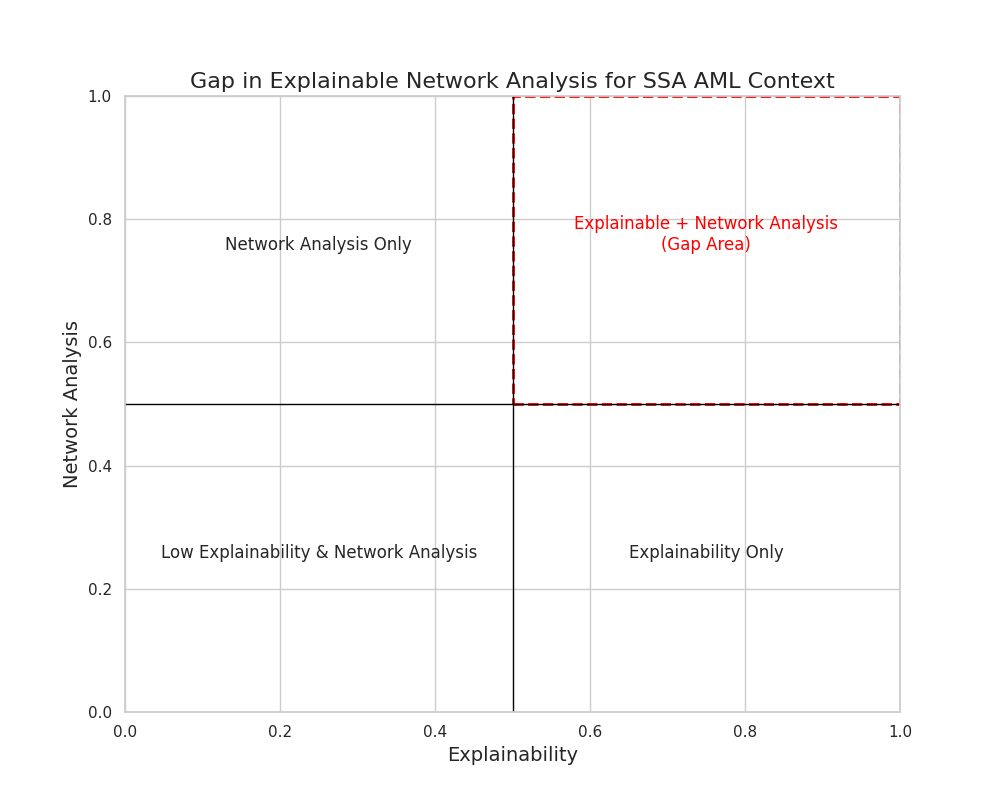
\includegraphics[width=0.82\textwidth]{images/networkAnalysisVsExplainability.png}
\caption{Conceptual positioning of the research: bridging the divide between high-capacity network analysis and regulatory explainable AI.}
\label{fig:conceptual_framework}
\end{figure}

\section{Summary}
This chapter established the theoretical foundations of money laundering, critiqued the structural breakdown of traditional rule engines, analyzed supervised and graph-based machine learning paradigms, and demonstrated the necessity of game-theoretic XAI for statutory compliance. The identified literature gaps justify the multi-layer hybrid framework formulated and empirically tested in the subsequent chapters.
